% LaTeX Template for Project Report, Version 2.0
% (Abstracted from a Major Project Report at CSED, NIT Calicut but can be
% modified easily to use for other reports also.)
%
% Released under Creative Commons Attribution license (CC-BY)
% Info: http://creativecommons.org/licenses/by/3.0/
%
% Created by: Kartik Singhal
% BTech CSE Batch of 2009-13
% NIT Calicut
% Contact Info: kartiksinghal@gmail.com
%
% It is advisable to learn the basics of LaTeX before using this template.
% A good resource to start with is http://en.wikibooks.org/wiki/LaTeX/
%
% All template fields are marked with a pair of angular brackets e.g. <title here>
% except for the ones defining citation names in ref.tex.
%
% Empty space after chapter/section/subsection titles can be used to insert text.
%
% Just compile this file using pdflatex after making all required changes.

\documentclass[12pt,a4paper]{article}
\usepackage[pdftex]{graphicx} %for embedding images
\usepackage{url} %for proper url entries
\usepackage[bookmarks, colorlinks=false, pdfborder={0 0 0}, pdftitle={Bao cao Do an 1: Tim kiem Heuristic voi A*}, pdfauthor={Hoai Hong Thanh}, pdfsubject={Co so tri tue nhan tao}, pdfkeywords={report}]{hyperref} %for creating links in the pdf version and other additional pdf attributes, no effect on the printed document
%\usepackage[final]{pdfpages} %for embedding another pdf, remove if not required
\usepackage[utf8]{vietnam}
\usepackage{booktabs}
\usepackage{float}
\usepackage{smartdiagram}
\usesmartdiagramlibrary{additions}
\usepackage[left=3cm, right=3cm, top=2cm, bottom=2cm]{geometry}
\usepackage{parskip}
\setlength{\parindent}{15pt}
\newcommand{\ra}[1]{\renewcommand{\arraystretch}{#1}}
\newcommand{\code}[1]{\texttt{#1}}

\usepackage{fancyhdr}
\setlength{\headheight}{15.2pt}
\pagestyle{fancy}
\lhead[<even output>]{Cơ sở trí tuệ nhân tạo}
\rhead[<even output>]{Tìm kiếm Heuristic với A*}

\begin{document}
\renewcommand\bibname{Tài liệu tham khảo} %Renames "Bibliography" to "References" on ref page

%include other pages
\begin{titlepage}

\begin{center}

% Top of the page

\includegraphics[width=0.18\textwidth]{hcmus.png}\\[0.1in]
\large{ĐẠI HỌC KHOA HỌC TỰ NHIÊN, ĐHQG-HCM\\KHOA CÔNG NGHỆ THÔNG TIN}\\
\normalsize
\vspace{4cm}
\textup{\large {CƠ SỞ TRÍ TUỆ NHÂN TẠO} \\ \Large Báo cáo Đồ án 1}\\[0.2in]

% Title
\huge \textbf {CHỦ ĐỀ:\\TÌM KIẾM HEURISTIC VỚI A*}\\[0.5in]
\vspace{4cm}



% Submitted by
\normalsize Nhóm thực hiện \\
\begin{table}[h]
\centering
\begin{tabular}{lr}\hline \\
1. Võ Nhật Vinh & 1612815\\
2. Hồng Thanh Hoài & 1612855\\ 
3. Huỳnh Minh Huấn & 1612858\\ \\ \hline
\end{tabular}
\end{table}

\vspace{.2in}
Giáo viên lý thuyết\\
{\textbf{PGS.TS Lê Hoài Bắc}}\\[0.1in]
Giáo viên hướng dẫn\\
{\textbf{Nguyễn Ngọc Thảo, Lê Ngọc Thành, Châu Ngọc Phương}}\\[0.2in]

\vfill
Tháng 10 năm 2018

\end{center}

\end{titlepage}
\newpage

\pagenumbering{roman} %numbering before main content starts
\cleardoublepage
%\pagebreak
\phantomsection
\addcontentsline{toc}{section}{Lời cảm ơn}
\section*{Lời cảm ơn}
\vspace{1.0in}
\begingroup
\setlength{\parindent}{0pt}
Trong quá trình thực hiện đồ án này, nhóm chúng em đã nhận được rất nhiều sự giúp đỡ cũng như hỗ trợ từ các thầy cô Trường Đại học Khoa học Tự nhiên, ĐHQG-HCM và các bạn bè
trong trường. Nhóm chúng em xin bày tỏ lòng cảm ơn chân thành đến mọi người vì đã hướng dẫn, chỉ bảo rất tận tình.

Đặc biệt, nhóm chúng em xin bày tỏ lòng biết ơn sâu sắc đến các thầy cô khoa Công nghệ
thông tin, cụ thể hơn là thầy Lê Hoài Bắc và các thầy cô hướng dẫn đã giảng dạy rất kĩ lưỡng để chúng em có thể hoàn thành tốt đồ án này.\par

Một lần nữa, chúng em xin bày tỏ lòng biết ơn sâu sắc đến với các thầy cô và bạn bè.\par

Tháng 10 năm 2018,\\
{Đại học Khoa học Tự nhiên, ĐHQG-HCM.}\\
\endgroup
\newpage

\tableofcontents


\newpage
\pagenumbering{arabic} %reset numbering to normal for the main content


\section{Giới thiệu nhóm và phân công công việc}
\subsection{Giới thiệu nhóm}
\textit{Nhóm gồm 3 thành viên.}   	
\begin{table*}[h]\centering
\ra{1.3}
\begin{tabular}{llll}\toprule
\textbf{STT} & \textbf{Họ và tên} & \textbf{MSSV} & \textbf{Email}\\\midrule
1 & Võ Nhật Vinh & 1612815 & \href{mailto:nhatvinhvo1998@gmail.com}{nhatvinhvo1998@gmail.com}\\
2 & Hồng Thanh Hoài & 1612855 & \href{mailto:hthoai1006@gmail.com}{hthoai1006@gmail.com}\\
3 & Huỳnh Minh Huấn & 1612858 & \href{mailto:minhhuanhuynh289@gmail.com}{minhhuanhuynh289@gmail.com}\\
\bottomrule
\end{tabular}
\end{table*}

\subsection{Phân công công việc}
%\begin{table*}[h]\centering
%\ra{1.3}
%\begin{tabular}{cllc}\toprule
%\textbf{STT} & \textbf{Họ và tên} & \textbf{Công việc} & \textbf{Hoàn thành}\\\midrule
%1 & Huỳnh Minh Huấn & Hàm \code{astar-search} & 100\%\\
%2 & Hồng Thanh Hoài & Hàm \code{main}, lớp \code{Cell} & 100\%\\
%3 & Võ Nhật Vinh & Lớp \code{PriorityQueue}, viết báo cáo và testcase & 100\%\\
%\bottomrule
%\end{tabular}
%\end{table*}


\begin{table}[h]\centering\ra{1.3}
\begin{tabular}{@{}cllcl@{}}
\toprule
\multicolumn{1}{l}{\textbf{STT}} & \textbf{Họ và tên}       & \textbf{Công việc}                                                                            & \multicolumn{1}{l}{\textbf{Mức độ hoàn thành}} &  \\ \toprule
1                       & Huỳnh Minh Huấn & Hàm \code{astar-search}                                                                     & 100\%                                 &  \\\midrule
2                       & Hồng Thanh Hoài & \begin{tabular}[c]{@{}l@{}}Hàm \code{main}\\ Lớp \code{Cell}\end{tabular}                          & 100\%                                 &  \\\midrule
3                       & Võ Nhật Vinh    & \begin{tabular}[c]{@{}l@{}}Lớp \code{PriorityQueue}\\ Viết testcases\\ Viết báo cáo\end{tabular} & 100\%                                 &  \\ \bottomrule
\end{tabular}
\end{table}
\newpage
\section{Giới thiệu đồ án}
\subsection{Thời gian và công cụ thực hiện}
\begin{itemize}
	\item[--] Thời gian thực hiện: từ ngày 10/10/2018 đến ngày 22/10/2018.
	\begin{itemize}
		\item[$\bullet$] 10/10/2018 – 14/10/2018: Tìm hiểu kiến thức liên quan.
		\item[$\bullet$] 14/10/2018 – 20/10/2018: Thiết kế thuật toán, class, hàm... và tiến hành code.
		\item[$\bullet$] 20/10/2018 – 22/10/2018: Tổng hợp source code, testing, release và viết báo cáo. 
	\end{itemize}
%\begin{table}[h]\centering\ra{1.3}
%\begin{tabular}{p{5cm} p{6cm}}
%\toprule
%Thời gian & Công việc \\ \midrule
%10/10/2018 – 14/10/2018 & Tìm hiểu kiến thức liên quan \\
%14/10/2018 – 20/10/2018 & Thiết kế thuật toán, class, hàm... và tiến hành code. \\
%20/10/2018 – 22/10/2018 & Tổng hợp source code, testing, release và viết báo cáo. \\ \bottomrule
%\end{tabular}
%\end{table}
	\item[--] Công cụ làm việc nhóm: Facebook.
	\item[--] Công cụ quản lý \textit{source code}: Github.
	\item[--] \textit{Text editor}: Visual Studio Code.
\end{itemize}
\subsection{Các bước thực hiện}
\begin{figure}[h]
  \centering
  \smartdiagramset{
    uniform color list=white!60!black for 6 items,
    back arrow disabled=true,
    module minimum width=2cm,
    module minimum height=2cm,
    module x sep=4cm,
    text width=3cm,
    additions={
      additional item offset=20mm,
      additional item width=2cm,
      additional item height=2cm,
      additional item text width=3cm,
      additional item shadow=drop shadow,
      additional item bottom color=white!60!black,
      additional item border color=gray,
      additional arrow color=gray,
    }}
  \smartdiagramadd[flow diagram:horizontal]{
    Tìm hiểu kiến thức liên quan, Thiết kế class - thủ tục - hàm, Phân chia công việc
  }{
    below of module1/Tổng hợp source code,below of module2/Testing,below of module3/Release
  }
  \smartdiagramconnect{->}{additional-module1/additional-module2,additional-module2/additional-module3}
  \begin{tikzpicture}[remember picture,overlay]% modified from p. 47 of manual
    \draw[additional item arrow type] (module3) |- ([yshift=-10mm]module1.south) -- (additional-module1);
  \end{tikzpicture}
  \vspace{40mm}\par
  %\caption{My diagram}\label{fig:diag}
\end{figure}
\newpage
\section{Nội dung đồ án}
\subsection{Sơ đồ UML}
\textit{Sơ đồ UML thể hiện thiết kế hàm, class.}
\begin{figure}[htb]
\centering
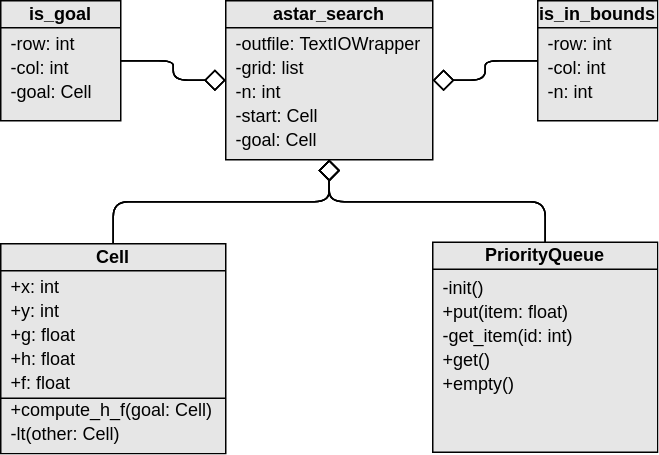
\includegraphics[width=0.98\textwidth]{uml.png} % e.g. insert ./image for image.png in the working directory, adjust scale as necessary
\end{figure}

\subsection{Các hàm chính}
\begin{itemize}
	\item \code{astar-search}
	\begin{itemize}
		\item Tham số đầu vào: \code{outfile} (chứa kết quả), \code{grid} (chứa bản đồ), \code{n} (kích thước bản đồ: n x n), \code{start} - \code{goal} (điểm xuất phát và điểm đích).
		\item Công dụng: Dùng thuật toán A* để tìm đường đi từ một điểm đến một điểm cho trước, trả về \textit{-1} nếu không tìm thấy đường đi.
	\end{itemize}
	
	\item \code{is-in-bounds}
	\begin{itemize}
		\item Tham số đầu vào: \code{row} - \code{col} (tọa độ của ô cần kiểm tra), \code{n} (kích thước bản đồ).
		\item Công dụng: Kiểm tra xem một ô có nằm trong bản đồ hay không.
	\end{itemize}
	
	\item \code{is-goal}
	\begin{itemize}
		\item Tham số đầu vào: \code{row} - \code{col} (tọa độ của ô cần kiểm tra), \code{goal} (ô đích).
		\item Công dụng: Kiểm tra xem một ô có phải là đích hay không.
	\end{itemize}
\end{itemize}

\subsection{Cấu trúc dữ liệu}
\begin{itemize}
	\item Class \code{Cell} với các thuộc tính:
	\begin{itemize}
		\item[+] \code{x}, \code{y}: tọa độ của ô trên bản đồ.
		\item[+] \code{g}: hàm chi phí đi từ điểm bắt đầu đến điểm hiện hành.
		\item[+] \code{h}: hàm heuristic ước lượng khoảng cách từ điểm hiện hành đến đích.
		\item[+] \code{f}: \code{f = g + h}.
	\end{itemize}
	\item \code{PriorityQueue}: hàng đợi ưu tiên.
\end{itemize}

\subsection{Thuật toán chính}
\textit{Thuật toán chính sử dụng là tìm kiếm A*.}
\begin{itemize}
	\item Bước 1: Nếu \code{start} và \code{goal} không nằm trong bản đồ hoặc là vật cản thì kết thúc thuật toán.
	\item Bước 2: Khởi tạo \code{open list}, khởi tạo \code{closed-list} với tất cả giá trị là \code{False}, và khởi tạo \code{parent-list} với tất cả các giá trị có tọa độ \code{(-1, -1)} và \code{f = FLOAT-MAX}. Đưa \code{start} vào \code{open-list}.
	\item Bước 3: Lặp khi \code{open-list} không rỗng:
	\begin{itemize}
		\item Lấy ra node có giá trị \code{f} thấp nhất trong \code{open-list}, gọi là \code{q}. Gán \code{True} cho vị trí của \code{q} trong \code{close list}.
		\item Nếu \code{q} là \code{goal}, tiến hành quay lui thông qua \code{parent-list} để tìm đường đi và kết thúc thuật toán.
		\item Khởi tạo 8 successor xung quanh lân cận 8 của \code{q}.
		\item Với mỗi successor:
		\begin{itemize}
			\item[+] Nếu successor nằm trong bản đồ, không phải là vật cản, và giá trị trong \code{closed-list} là \code{False} thì tiến hành tính \code{g}, \code{h}, \code{f} cho successor này.
			\item[+] Nếu \code{parent} của successor này có \code{f = FLOAT-MAX} hoặc \code{f} lớn hơn \code{f} của successor, ta gán \code{parent} mới cho successor với tọa độ là tọa độ của \code{q}, \code{f} là \code{f} của successor. Và thêm successor này vào \code{open-list}.
		\end{itemize}
	\end{itemize}
	
	\item Bước 4: Nếu \code{open-list} đã rỗng mà chưa tìm thấy đường đi thì kết thúc thuật toán.
	
\end{itemize}
\newpage
\section{Kiểm thử}
\textit{Sử dụng 10 testcase với ba đặc trưng khác nhau là: kích thước nhỏ, kích thước lớn, và không có đường đi.}

\subsection{Testcase với kích thước nhỏ}

\begin{figure}[H]
\centering
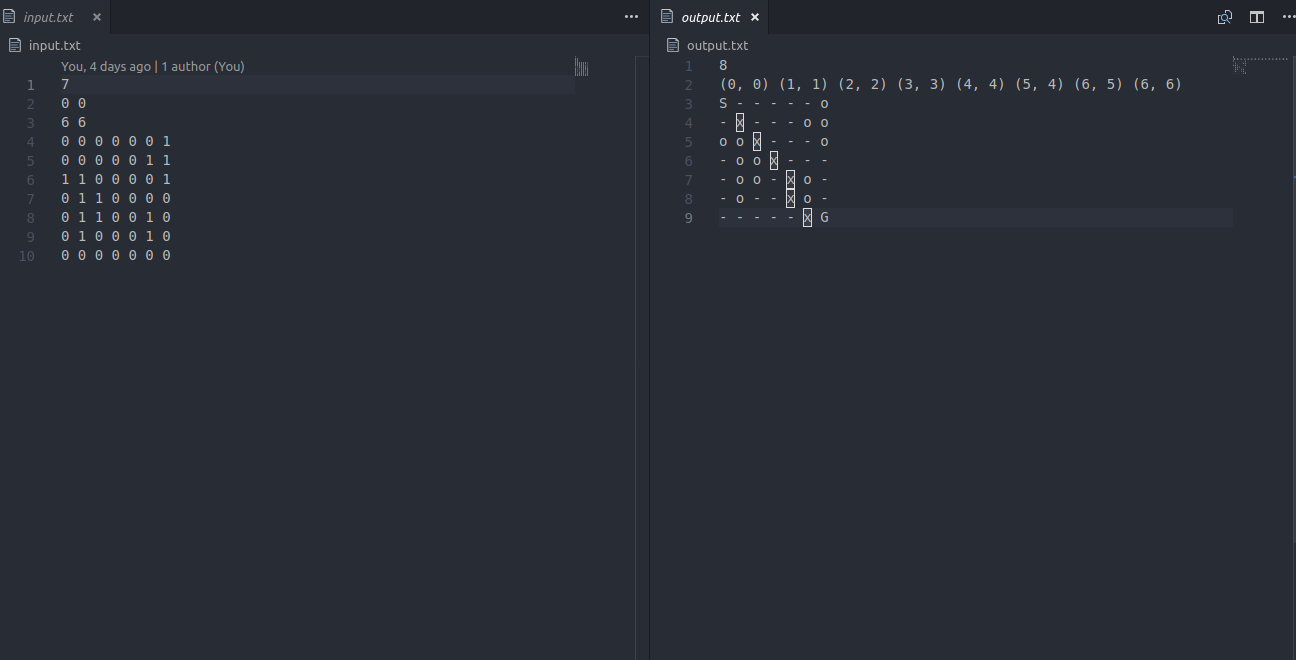
\includegraphics[width=0.98\textwidth]{t0.png}
\caption{Testcase 8x8.}
\end{figure}

\begin{figure}[H]
\centering
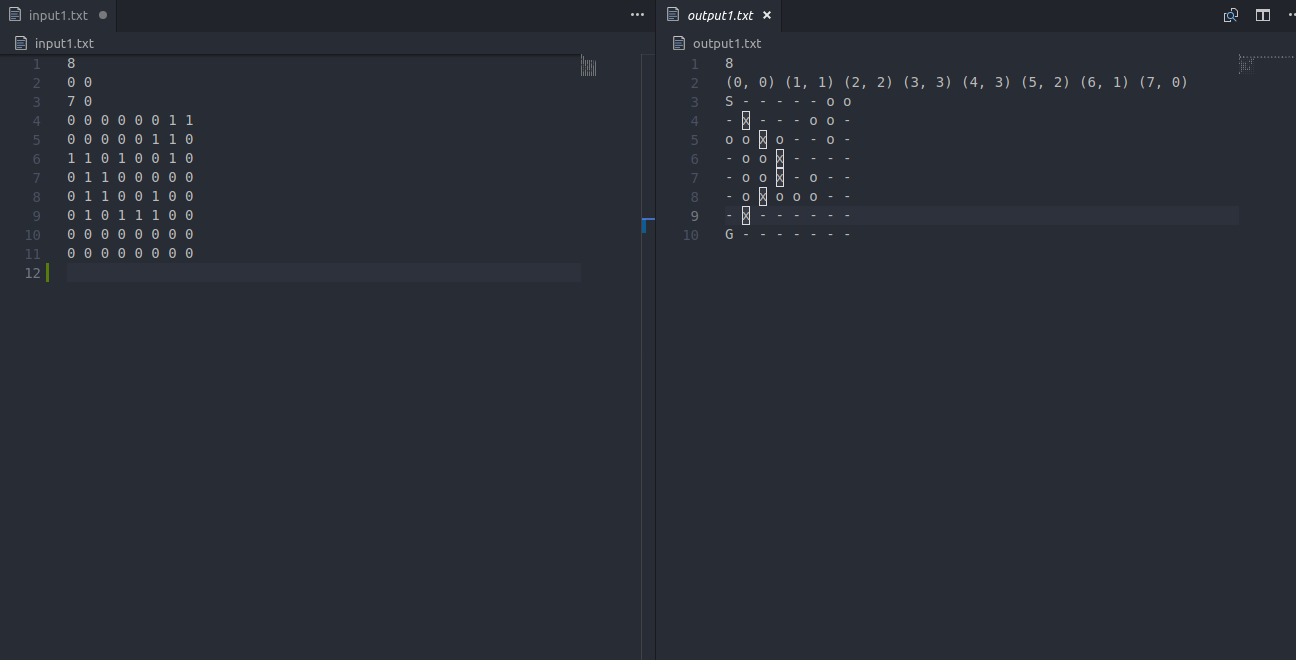
\includegraphics[width=0.98\textwidth]{t1.png}
\caption{Testcase 8x8.}
\end{figure}

\begin{figure}[H]
\centering
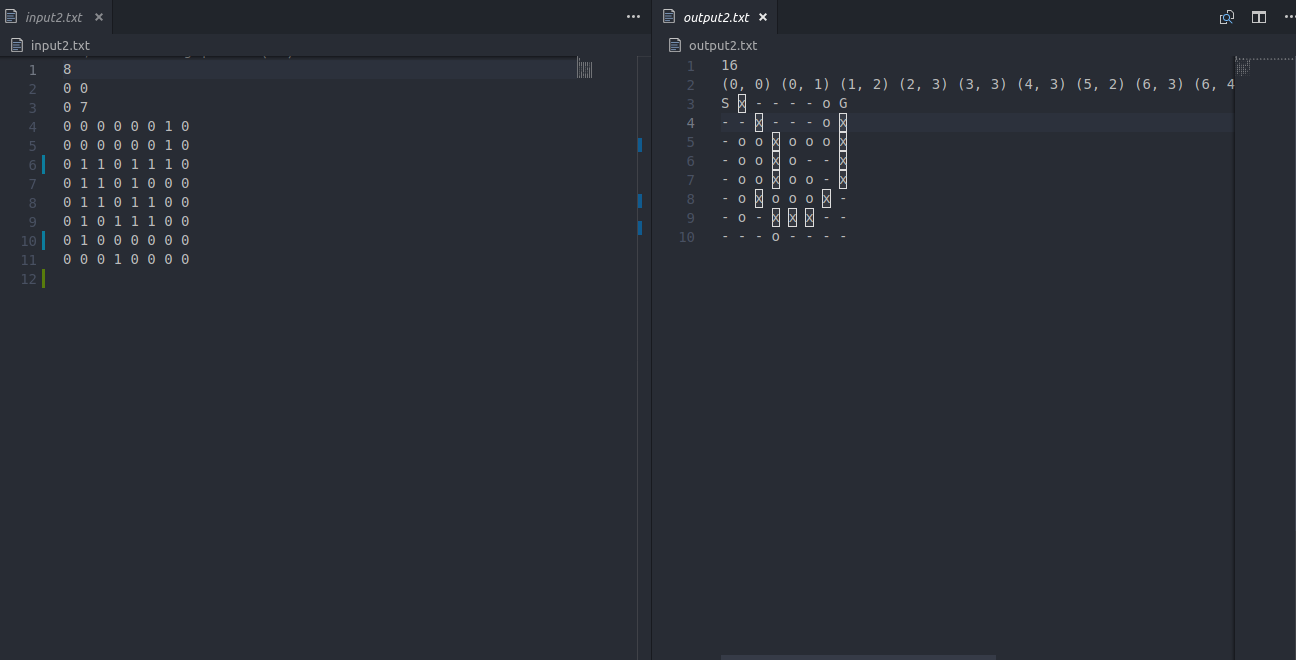
\includegraphics[width=0.98\textwidth]{t2.png}
\caption{Testcase 8x8.}
\end{figure}

\begin{figure}[H]
\centering
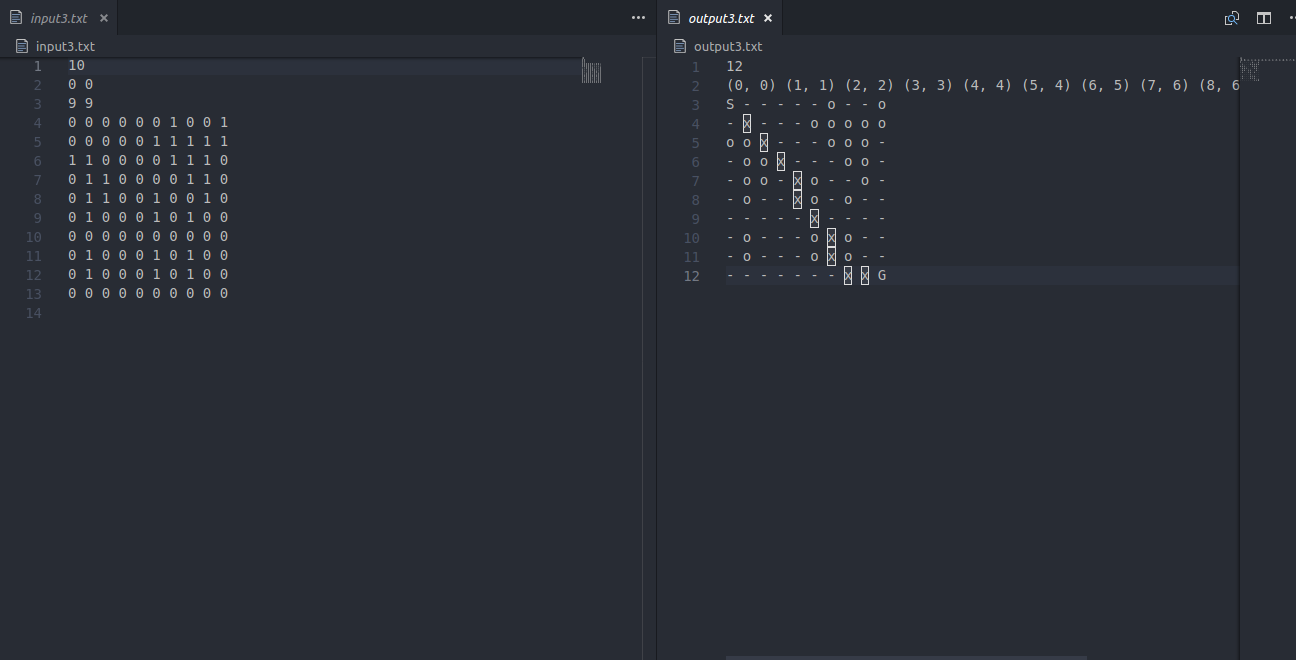
\includegraphics[width=0.98\textwidth]{t3.png}
\caption{Testcase 10x10.}
\end{figure}

\subsection{Testcase với kích thước lớn}

\begin{figure}[H]
\centering
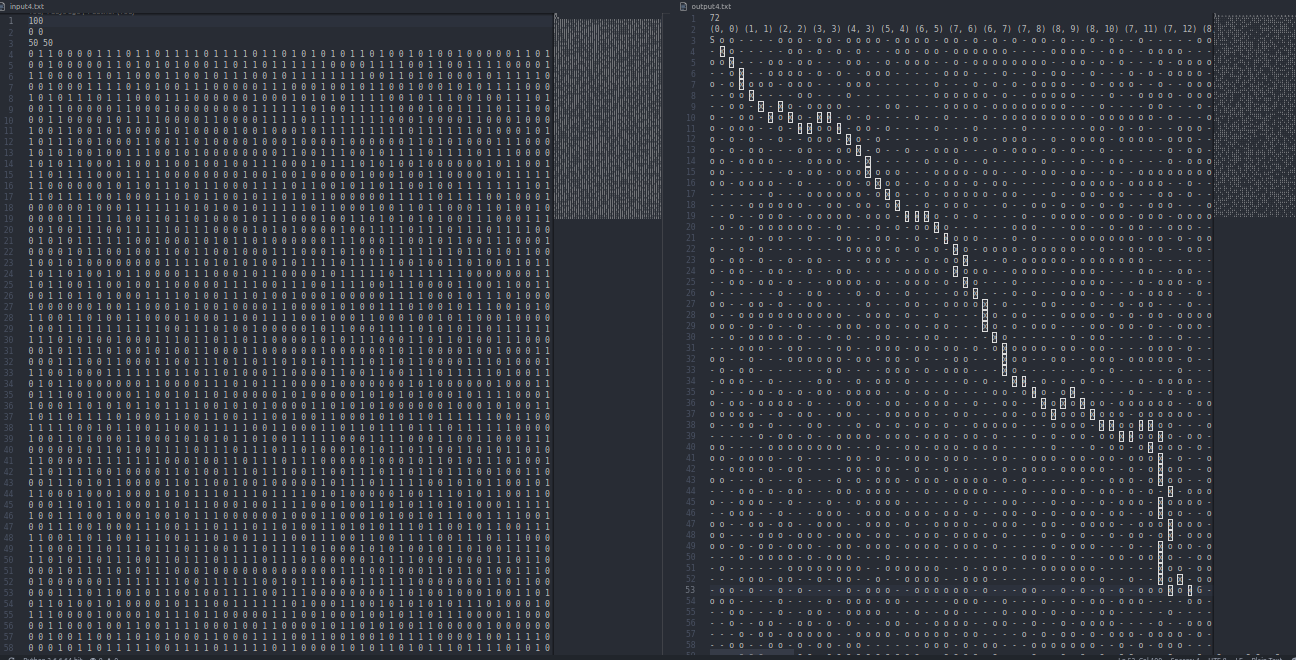
\includegraphics[width=0.98\textwidth]{t4.png}
\caption{Testcase 100x100.}
\end{figure}

\begin{figure}[H]
\centering
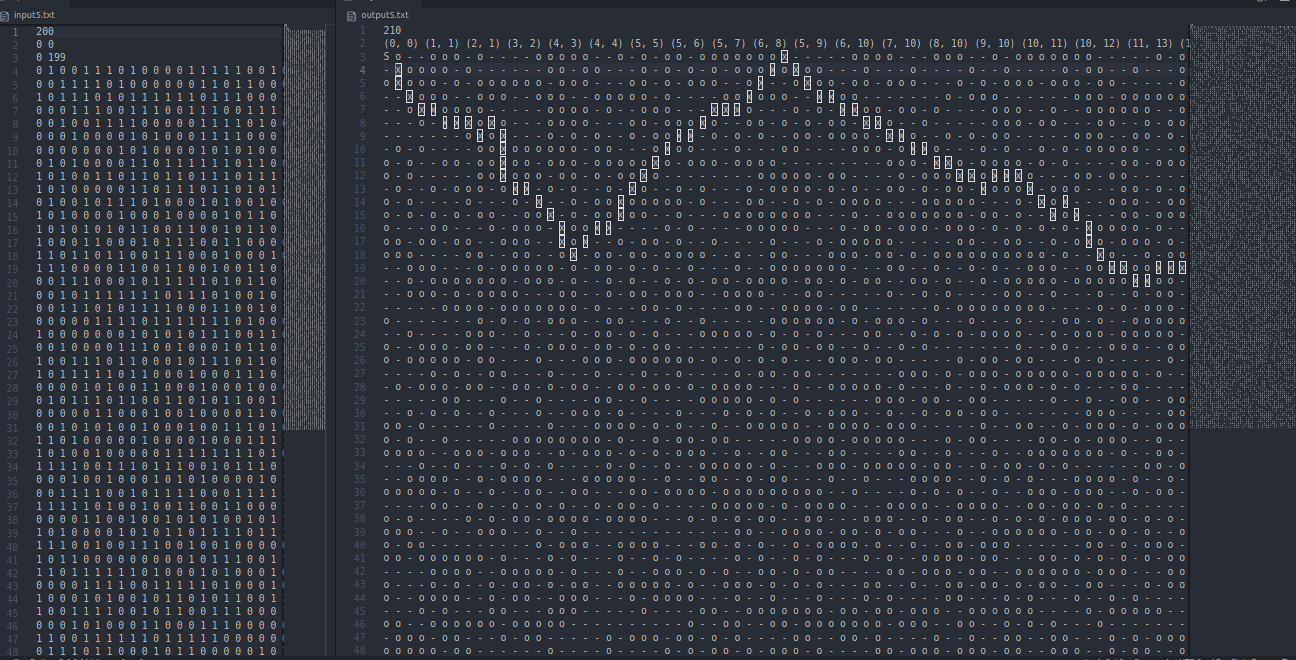
\includegraphics[width=0.98\textwidth]{t5.png}
\caption{Testcase 200x200.}
\end{figure}

\begin{figure}[H]
\centering
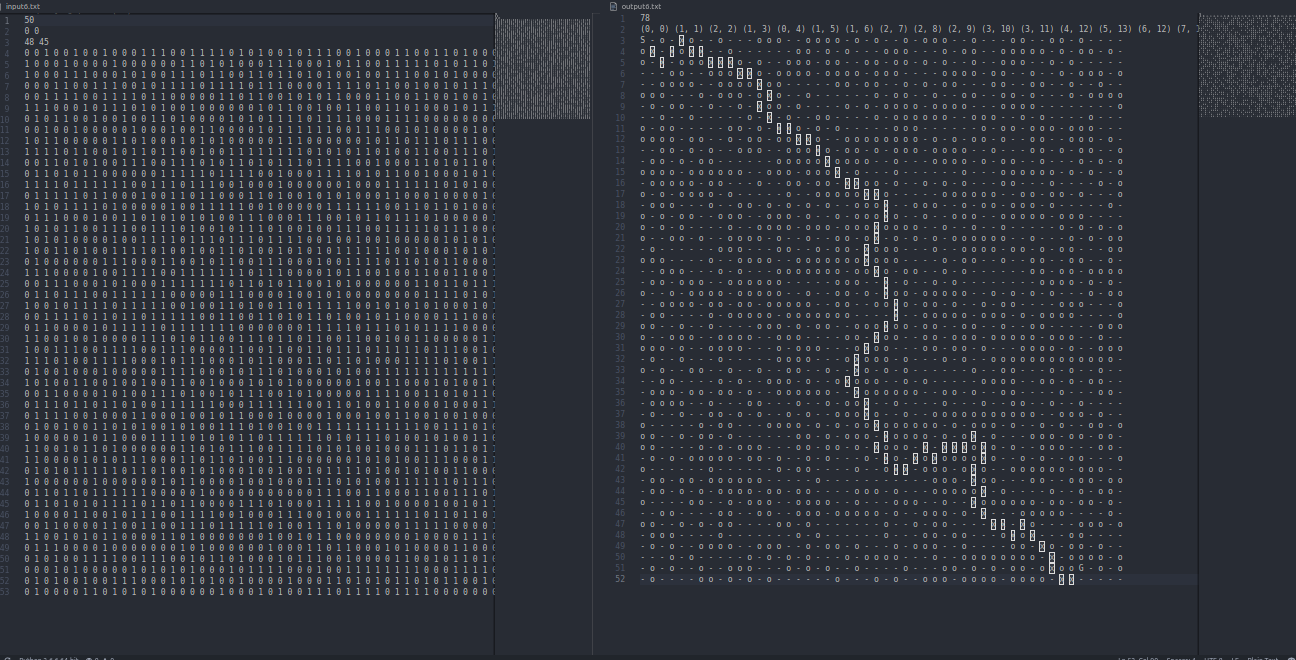
\includegraphics[width=0.98\textwidth]{t6.png}
\caption{Testcase 50x50.}
\end{figure}

\subsection{Testcase không có đường đi từ \code{start} đến \code{goal}}

\begin{figure}[H]
\centering
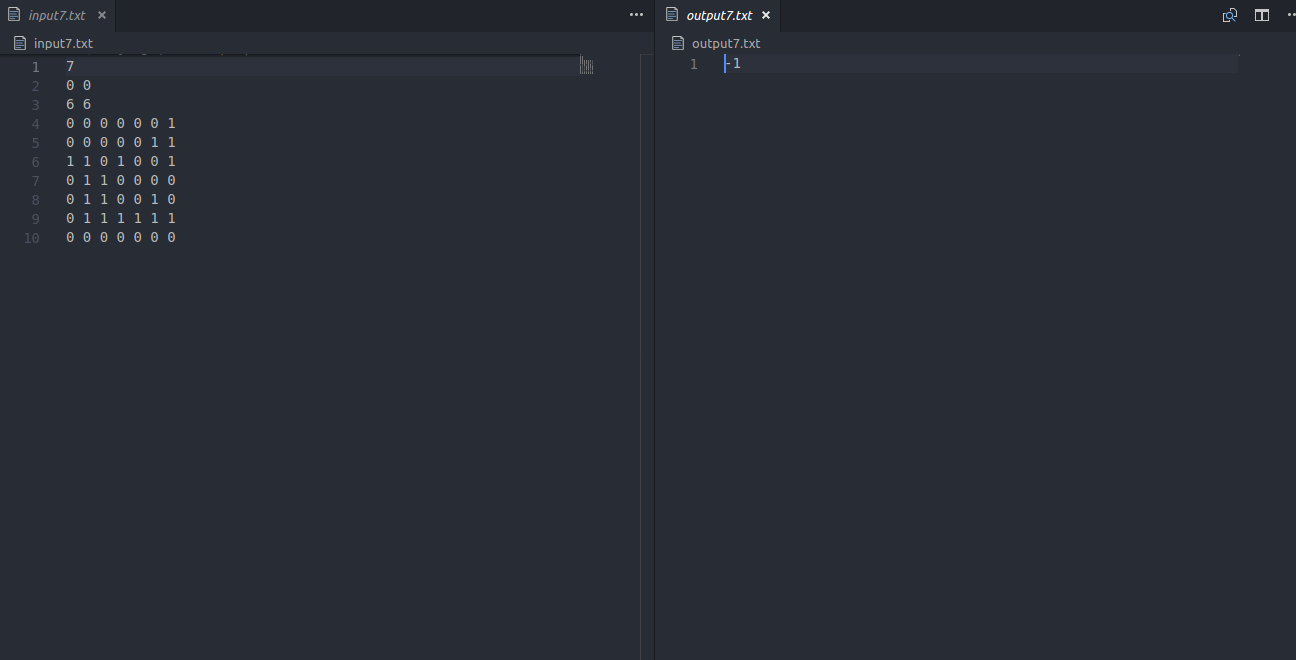
\includegraphics[width=0.98\textwidth]{t7.png}
\caption{Testcase 7x7.}
\end{figure}

\begin{figure}[H]
\centering
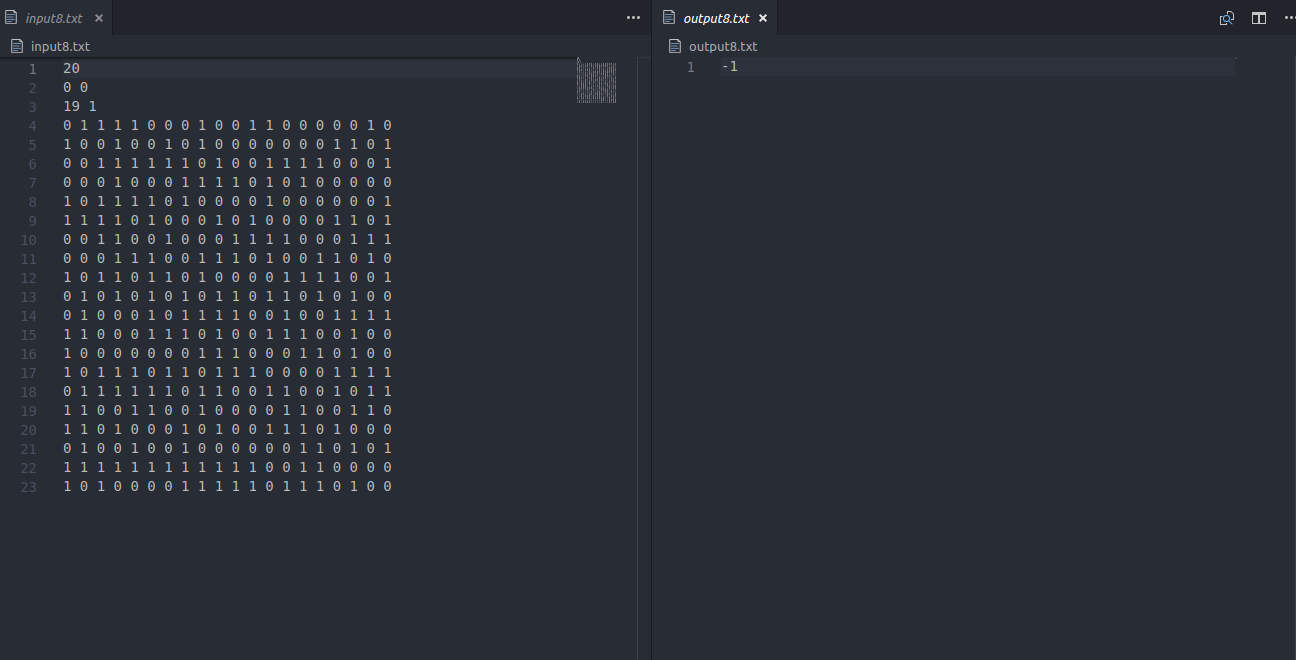
\includegraphics[width=0.98\textwidth]{t8.png}
\caption{Testcase 20x20.}
\end{figure}

\begin{figure}[H]
\centering
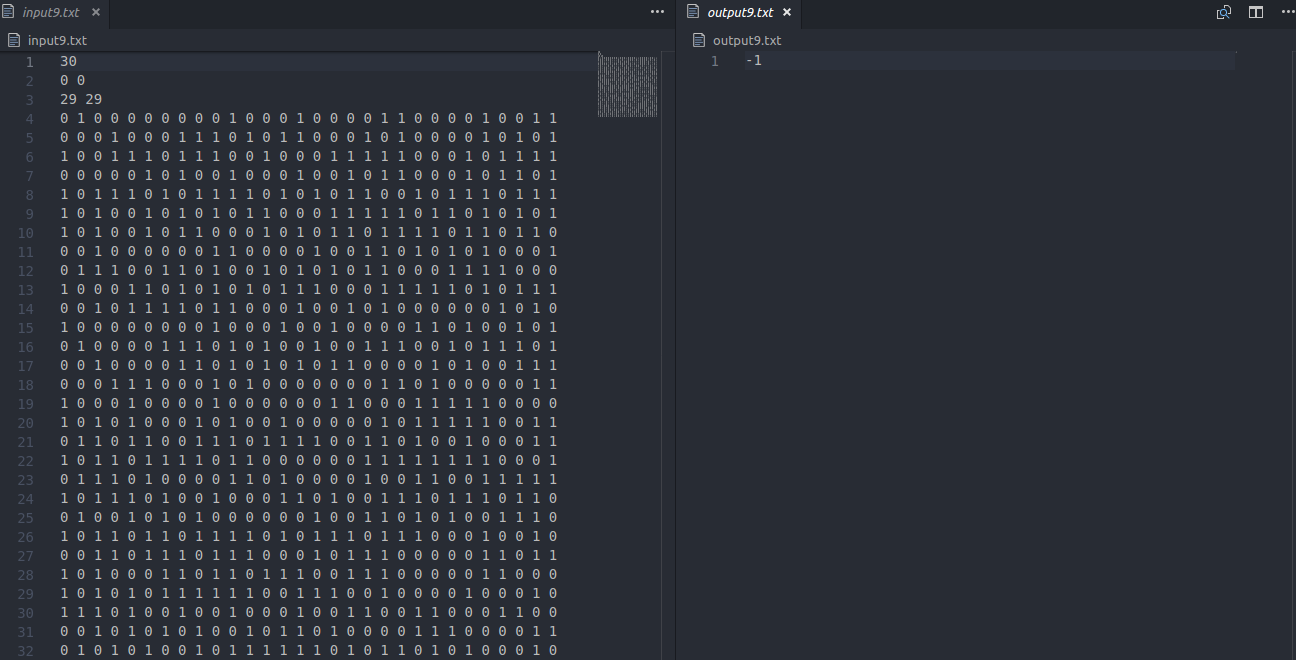
\includegraphics[width=0.98\textwidth]{t9.png}
\caption{Testcase 30x30.}
\end{figure}

\newpage
\section{Đánh giá và tổng kết quá trình}

\subsection{Mức độ hoàn thành của đồ án}

\begin{table}[H]\centering\ra{1.3}
\begin{tabular}{@{}clc@{}}
\toprule
\textbf{STT} & \multicolumn{1}{c}{\textbf{Nội dung}} & \textbf{Hoàn thành} \\ \midrule
1 & Tìm hiểu kỹ kiến thức, phân chia công việc rõ ràng. & 100\% \\
2 & Vẽ sơ đồ UML, mô tả cấu trúc dữ liệu, thuật toán cài đặt. & 100\% \\
3 & Trình bày code sạch sẽ, comment và docstring đầy đủ. & 100\% \\
4 & Sử dụng testcase với ba đặc trưng khác nhau. & 100\% \\
5 & Kết quả đúng với yêu cầu đồ án. & 100\% \\ \midrule
\multicolumn{2}{c}{\textbf{Mức độ hoàn thành tổng thể của đồ án:}} & \textbf{100\%} \\ \bottomrule
\end{tabular}
\end{table}

\subsection{Những vấn đề chưa thực hiện được}
Nhóm đã thực hiện đầy đủ những yêu cầu của đồ án. Trong quá trình hoàn thành đồ án có phát sinh những vấn đề gây khó khăn nhưng nhóm đã giải quyết được.

\newpage


\cleardoublepage
%\pagebreak
\phantomsection
\addcontentsline{toc}{section}{Tài liệu tham khảo}
\begin{thebibliography}{99}

\bibitem{a1}Red Blob Games, \textit{\href{https://www.redblobgames.com/pathfinding/a-star/introduction.html}{Introduction to A*}}.

\bibitem{a2}Rosetta Code, \textit{\href{https://rosettacode.org/wiki/A*_search_algorithm}{A* search algorithm}}.

\bibitem{a3}Wikipedia, \textit{\href{https://en.wikipedia.org/wiki/A*_search_algorithm}{A* search algorithm}}.

\bibitem{a4}PGS.TS Lê Hoài Bắc, \textit{\href{https://drive.google.com/drive/folders/1Jre3ev47bMdiNgA3Qi26fpVJ5tFOBrx1}{Slide bài giảng về Heuristic Search}}.

\bibitem{a5}PyTutorials, \textit{\href{https://www.youtube.com/watch?v=lOIJIk_maO4}{Convert PY to EXE}}.

\end{thebibliography}


\end{document}
